\documentclass{article}
\usepackage{graphicx}
\usepackage{geometry}
\usepackage{hyperref}
\usepackage{booktabs}
\usepackage{subcaption}
\usepackage{amsmath}

\geometry{
    a4paper,
    margin=0.7in
}

\hypersetup{
    colorlinks=true,
    linkcolor=blue,
    filecolor=magenta,      
    urlcolor=cyan,
}

\title{SNN Surrogate Gradient \texttt{tri} $\beta$ Parameter Comparison\\Robustness Sweep under Data Heterogeneity ($f \le 1$)}
\author{ByzFL SNN Benchmark}
\date{\today}

\begin{document}

\maketitle

\section{Introduction}
This document presents a comparison of the Spiking Neural Network (SNN) robustness on the MNIST dataset using different scaling factors $\beta$ for the Triangular (\texttt{tri}) surrogate gradient. The evaluation spans:
\begin{itemize}
    \item \textbf{Surrogate Gradient Parameter}: $\beta \in \{0.5, 0.75, 1.0, 1.25, 1.5\}$
    \item \textbf{Byzantine Nodes}: $f \in \{0, 1\}$ out of $N=10$ honest nodes
    \item \textbf{Data Heterogeneity}: Non-IID levels $\gamma \in \{1.0, 0.66, 0.33, 0.0\}$
    \item \textbf{Attacks}: Worst-case outcome across SignFlipping and Optimal A Little Is Enough (\texttt{Optimal\_ALittleIsEnough\_neg1})
    \item \textbf{Aggregators}: Best aggregated result across Centered Clipping and Geometric Median (pre-aggregated with NNM and ARC).
\end{itemize}

\section{Aggregated Test Accuracy Heatmaps}
The figure below displays the aggregated test accuracy heatmaps for each tested $\beta$ parameter value for $f \le 1$.

\begin{figure}[htbp]
    \centering
    \begin{subfigure}[b]{0.48\textwidth}
        \centering
        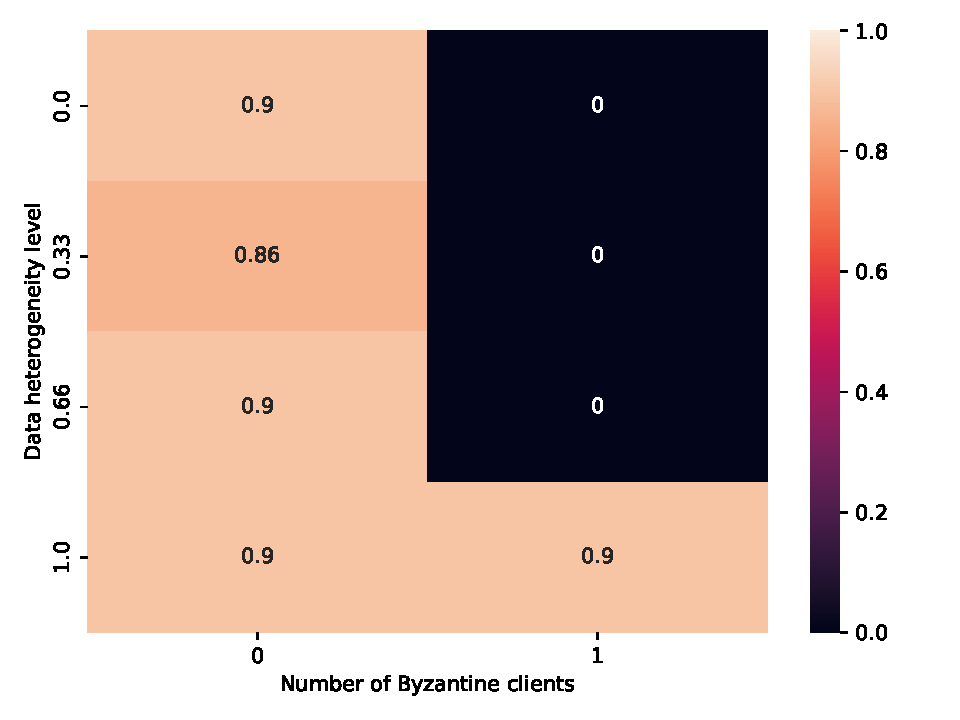
\includegraphics[width=\textwidth]{heatmap_tri_beta_0_5.pdf}
        \caption{$\beta = 0.5$}
        \label{fig:beta_0_5}
    \end{subfigure}
    \hfill
    \begin{subfigure}[b]{0.48\textwidth}
        \centering
        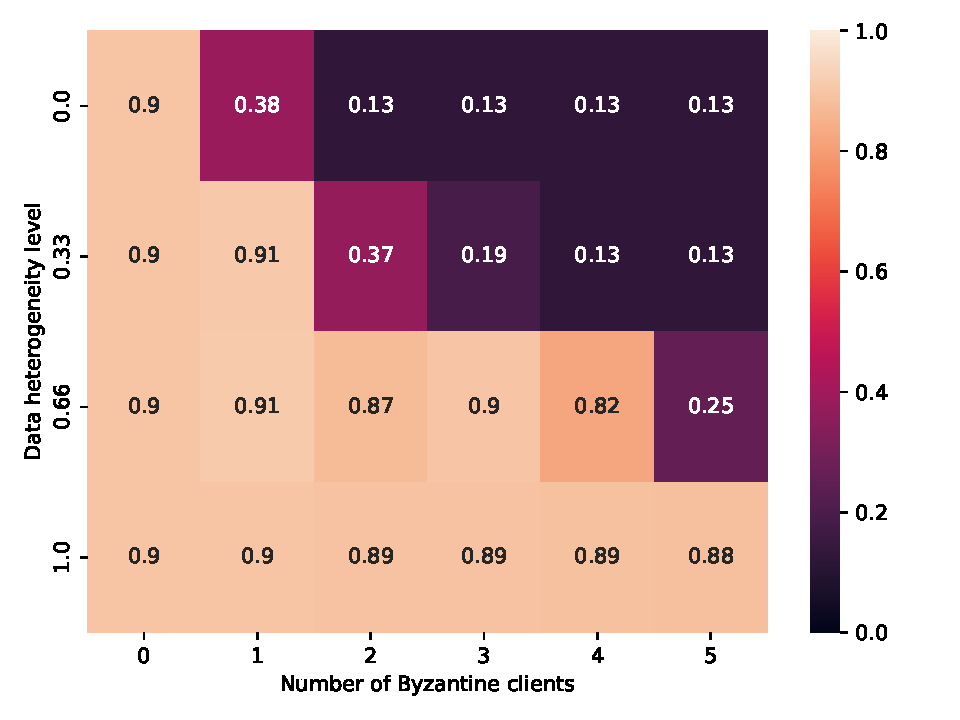
\includegraphics[width=\textwidth]{heatmap_tri_beta_0_75.pdf}
        \caption{$\beta = 0.75$}
        \label{fig:beta_0_75}
    \end{subfigure}
    
    \vspace{0.3cm}
    
    \begin{subfigure}[b]{0.48\textwidth}
        \centering
        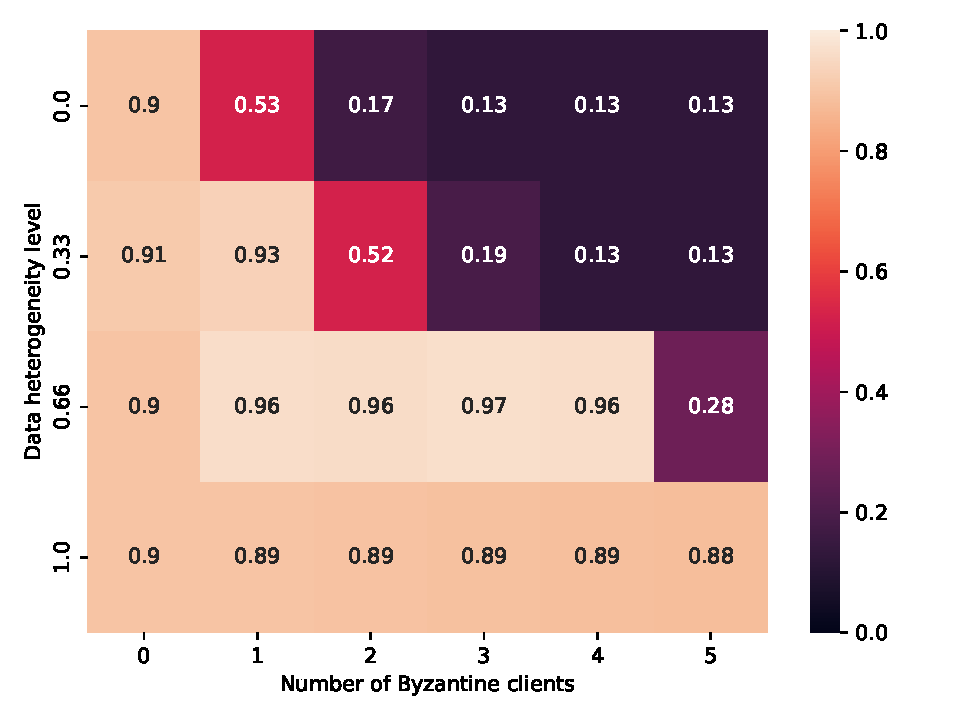
\includegraphics[width=\textwidth]{heatmap_tri_beta_1_0.pdf}
        \caption{$\beta = 1.0$}
        \label{fig:beta_1_0}
    \end{subfigure}
    \hfill
    \begin{subfigure}[b]{0.48\textwidth}
        \centering
        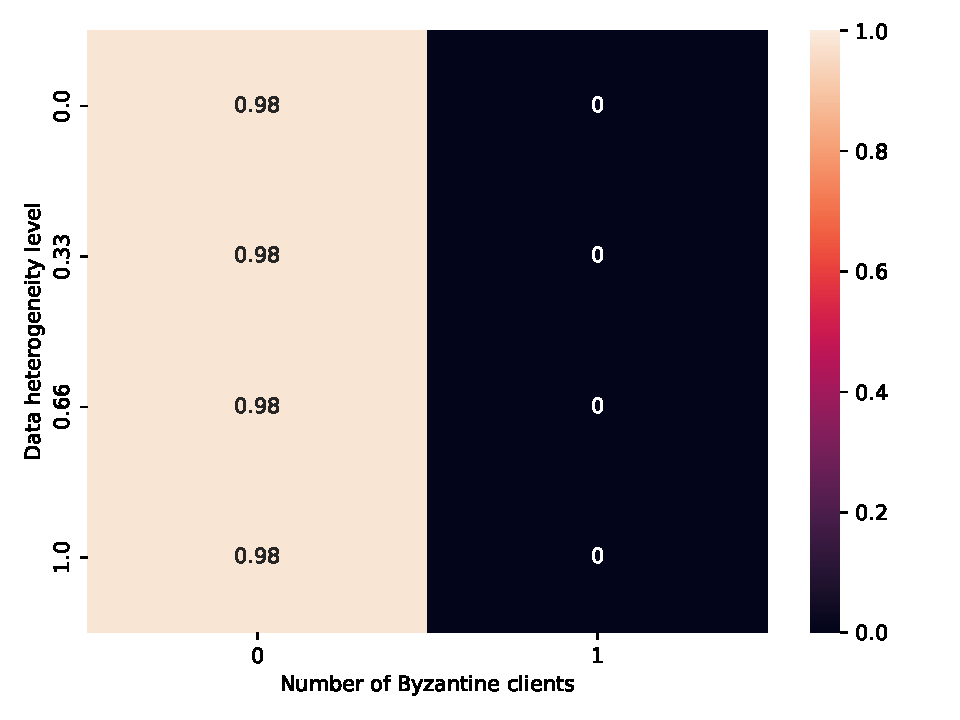
\includegraphics[width=\textwidth]{heatmap_tri_beta_1_25.pdf}
        \caption{$\beta = 1.25$}
        \label{fig:beta_1_25}
    \end{subfigure}
    
    \vspace{0.3cm}
    
    \begin{subfigure}[b]{0.48\textwidth}
        \centering
        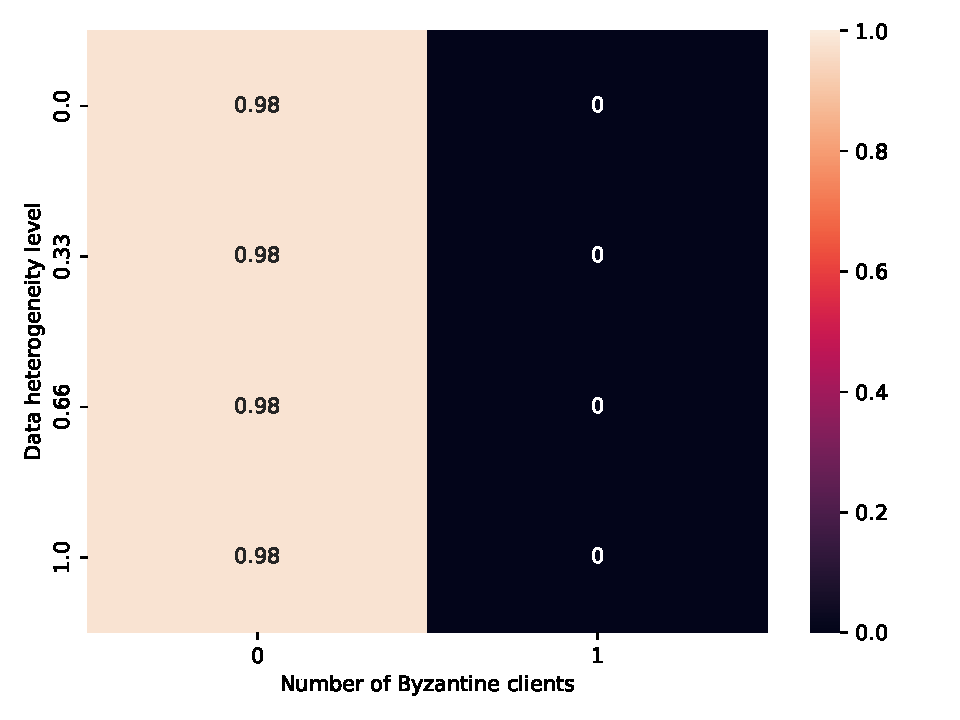
\includegraphics[width=\textwidth]{heatmap_tri_beta_1_5.pdf}
        \caption{$\beta = 1.5$}
        \label{fig:beta_1_5}
    \end{subfigure}
    
    \caption{Aggregated Test Accuracy Heatmaps across different surrogate gradient $\beta$ values for SNN ($f \le 1$).}
    \label{fig:tri_beta_heatmaps}
\end{figure}

\newpage

\section{Quantitative Performance Summary}
Table~\ref{tab:summary} compares the overall performance metrics for each $\beta$ parameter value. The metrics include the average accuracy across all 8 cells in the grid, and the worst-case accuracy.

\begin{table}[htbp]
    \centering
    \caption{Performance Summary for Different Surrogate Gradient scaling values ($\beta$).}
    \label{tab:summary}
    \begin{tabular}{lcc}
        \toprule
        \textbf{Surrogate Scaling ($\beta$)} & \textbf{Average Accuracy} & \textbf{Worst-case Accuracy} \\
        \midrule
        $\beta = 0.5$ & 55.62\% & 0.00\% \\
        $\beta = 0.75$ & 56.03\% & 0.00\% \\
        $\beta = 1.0$ & 45.02\% & 0.00\% \\
        $\beta = 1.25$ & 49.06\% & 0.00\% \\
        $\beta = 1.5$ & 48.95\% & 0.00\% \\
        \bottomrule
    \end{tabular}
\end{table}

\section{Detailed Grid Tables for each $\beta$}
This section lists the exact aggregated test accuracies for each data heterogeneity level ($\gamma$) and number of Byzantine clients ($f \in \{0, 1\}$).

\subsection{Surrogate scaling $\beta = 0.5$}
\begin{table}[htbp]
    \centering
    \begin{tabular}{ccc}
        \toprule
        & \textbf{f = 0} & \textbf{f = 1} \\
        \midrule
        $\gamma = 1.0$ & 89.77\% & 89.83\% \\
        $\gamma = 0.66$ & 89.82\% & 0.00\% \\
        $\gamma = 0.33$ & 85.70\% & 0.00\% \\
        $\gamma = 0.0$ & 89.82\% & 0.00\% \\
        \bottomrule
    \end{tabular}
\end{table}
\subsection{Surrogate scaling $\beta = 0.75$}
\begin{table}[htbp]
    \centering
    \begin{tabular}{ccc}
        \toprule
        & \textbf{f = 0} & \textbf{f = 1} \\
        \midrule
        $\gamma = 1.0$ & 89.69\% & 89.57\% \\
        $\gamma = 0.66$ & 89.69\% & 0.00\% \\
        $\gamma = 0.33$ & 89.69\% & 0.00\% \\
        $\gamma = 0.0$ & 89.62\% & 0.00\% \\
        \bottomrule
    \end{tabular}
\end{table}
\subsection{Surrogate scaling $\beta = 1.0$}
\begin{table}[htbp]
    \centering
    \begin{tabular}{ccc}
        \toprule
        & \textbf{f = 0} & \textbf{f = 1} \\
        \midrule
        $\gamma = 1.0$ & 89.62\% & 0.00\% \\
        $\gamma = 0.66$ & 89.63\% & 0.00\% \\
        $\gamma = 0.33$ & 91.25\% & 0.00\% \\
        $\gamma = 0.0$ & 89.64\% & 0.00\% \\
        \bottomrule
    \end{tabular}
\end{table}
\subsection{Surrogate scaling $\beta = 1.25$}
\begin{table}[htbp]
    \centering
    \begin{tabular}{ccc}
        \toprule
        & \textbf{f = 0} & \textbf{f = 1} \\
        \midrule
        $\gamma = 1.0$ & 98.12\% & 0.00\% \\
        $\gamma = 0.66$ & 98.13\% & 0.00\% \\
        $\gamma = 0.33$ & 98.12\% & 0.00\% \\
        $\gamma = 0.0$ & 98.10\% & 0.00\% \\
        \bottomrule
    \end{tabular}
\end{table}
\subsection{Surrogate scaling $\beta = 1.5$}
\begin{table}[htbp]
    \centering
    \begin{tabular}{ccc}
        \toprule
        & \textbf{f = 0} & \textbf{f = 1} \\
        \midrule
        $\gamma = 1.0$ & 97.90\% & 0.00\% \\
        $\gamma = 0.66$ & 97.89\% & 0.00\% \\
        $\gamma = 0.33$ & 97.92\% & 0.00\% \\
        $\gamma = 0.0$ & 97.87\% & 0.00\% \\
        \bottomrule
    \end{tabular}
\end{table}

\end{document}
